\documentclass[conference]{IEEEtran}
\IEEEoverridecommandlockouts
\usepackage{cite}
\usepackage{amsmath,amssymb,amsfonts}
\usepackage{algorithmic}
\usepackage{graphicx}
\usepackage{textcomp}
\usepackage{xcolor}
\usepackage{babel}

%added packages
\usepackage{caption}
\usepackage{subcaption}
\usepackage[hidelinks]{hyperref}
\def\BibTeX{{\rm B\kern-.05em{\sc i\kern-.025em b}\kern-.08em
    T\kern-.1667em\lower.7ex\hbox{E}\kern-.125emX}}
\begin{document}

\title{Skin Lesion Classification Using Machine Learning\\}

% #NOTE without university name (which is a bit trivial), this fits into one line

\author{\IEEEauthorblockN{Sai Preetham Sata}
\IEEEauthorblockA{\textit{Hamburg University of Technology}\\
sai.sata@tuhh.de}
\and
\IEEEauthorblockN{Harsha Bajje Thippeswamy}
\IEEEauthorblockA{\textit{Hamburg University of Technology}\\
harsha.bajje.thippeswamy@tuhh.de }
\and
\IEEEauthorblockN{Sebastian Engelhardt}
\IEEEauthorblockA{\textit{Hamburg University of Technology}\\
sebastian.engelhardt@tuhh.de}
\and
\IEEEauthorblockN{Tim Neuwerk}
\IEEEauthorblockA{\textit{Hamburg University of Technology}\\
tim.neuwerk@tuhh.de}
}

\maketitle
%\tableofcontents
\begin{abstract}[TN]
In this work we present two different methods for the ISIC 2019 Skin Lesion Classification Challenge. The goal is to predict the class of a skin lesion based on dermoscopic images. Herefor a dataset of around 25000 images of eight different classes are given for training. Furthermore for most images additional meta data is provided which consists of information of the age and gender of the patient and the position of the skin lesion on the human body. The final test set contains an additional ninth class, which is unknown.\newline
In our first approach we are using Support Vector Machine for the classification. Therefor we also consider image preprocessing and feature extraction. These features describe the shape and texture of the lesion.\newline
In our second approach we are using deep learning to face the problem. We used the pretrained Convolutional Neural Network EfficientNet and applied transfer learning.\newline
The second approach promises significantly better results than the first. We achieved a sensitivity score based on the training data of 85.31\%.
\end{abstract}

% Include files with content here, this makes it a bit cleaner

% !TEX root = Skin_Lesion_Classification_Using_Machine_Learning.tex

\section{Introduction [TN, SE]}\label{sec:introduction}
%#TODO: Motivation for Machine Learning, describing the unknown class problem
Skin cancer is one of the most common types of cancer. It makes up more then half of the worldwide cancer diagnoses. Melanoma is the most dangerous type of skin cancer that can arise through different causes. A mole can change over time with an increase in size, irregular edges, change in color, itchiness or skin breakdown \cite{Zaqout19}. The primary cause of melanoma is the influence of ultraviolet light exposure from the sun or other sources like tanning devices. Its incidence and mortality rates have been increasing in the last decades \cite{Lens04} and therefore it represents an important public health problem. In 2012 out of 232,000 people that were diagnosed with Melanoma 55,000 people died. \\
However, if skin cancer is diagnosed in an early stage, it has very high curing rates. To detect cancerous skin dermatologists usually evaluate a skin lesion with the so called ABCD rule \cite{Stolz94}. In the first step the "\textbf{a}symmetry, \textbf{b}order, \textbf{c}olors, and \textbf{d}iameter" criteria are approximately estimated. In the second step each criteria is multiplied by a given weight factor to get the total dermoscopy score. This shows the importance of the shape and texture of the lesion in skin cancer diagnoses.\newline \newline
In this work we will use machine learning techniques to classify the type of skin lesion based on skin lesion images. For the required data we use the ``ISIC 2019: Training'' dataset that was published by the International Skin Imaging Collaboration (ISIC). This dataset contains 25,331 images of 8 different types of skin lesions. The test dataset also contains additional skin images that don't fall in any of there categories. Those images are referred to as unknown. 
The dataset is composed of three separate sources. Part of the data originates from the HAM1000 dataset \cite{HAM10000}. Those images are of size $600 \times 450$ and were manually cropped around the lesion by the dataset creators. Some of the images are also preprocessed by histogram equalization. % #TODO where to put the citation? This is all based on \cite{HAM10000}
The second dataset is the BCN20000 dataset \cite{bcn20000} containing high resolution images ($1024 \times 1024$). Not all images of that dataset are cropped, meaning there are images present with large black borders and the skin only visible in a circle in the middle. The last dataset is the MSK dataset \cite{MSK_Data} with images of different sizes originating from several sources. 
Table \ref{tab:data} shows the name of the lessions together with the number of images of these classes in the training dataset.

\begin{table}[ht]
    \caption{Number of samples per class in the training dataset}
    \begin{center}
    \begin{tabular}{c|c}
        \hline
        \textbf{Lesion}&\textbf{Number of samples} \\
        % \hline
        0-Melanoma &  4522 \\
        % \hline
        1-Melanocytic nevus & 12875  \\
        % \hline
        2-Basal cell carcinoma & 3323 \\
        % \hline
        3-Actinic keratosis & 867 \\
        % \hline
        4-Benign keratosis & 2624 \\
        % \hline
        5-Dermatofibroma & 239 \\
        % \hline
        6-Vascular lesion & 253 \\
        % \hline
        7-Squamous cell carcinoma & 628 \\
        % \hline
        8-Unknows & 0 \\
        \hline
    \end{tabular}
    \label{tab:data}
    \end{center}
\end{table}

As seen in the table, the dataset is heavily imbalanced. To get meaningful evaluation results, we rate our approaches using the  balanced multi-class accuracy, wich is equivalent to the macro-average sensitivity, as our main metric \cite{Mosley2013}. 
% #TODO maybe move to a better location?

Four images and the belonging classes are illustrated in figure \ref{fig:dataset}.
% #TODO select more meaningful images (with hair, cropped/not cropped, ...)
\begin{figure}
	\begin{subfigure}{.24\textwidth}
		\centering
		% include first image
		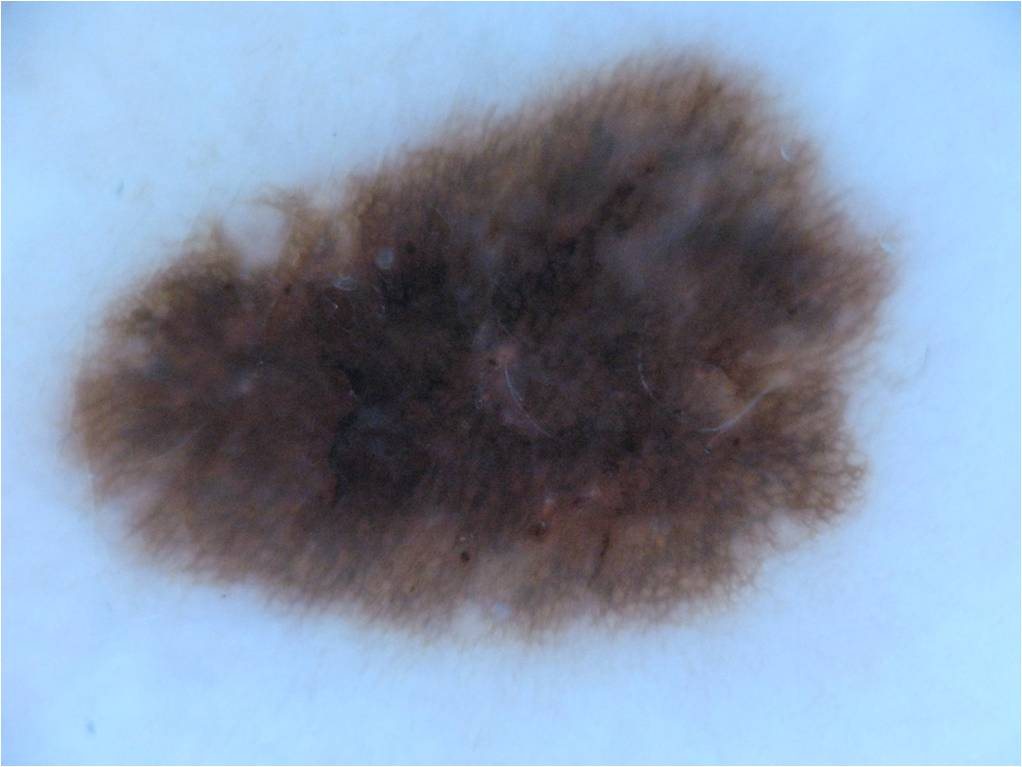
\includegraphics[width=.9\linewidth]{pictures/ISIC_0000000.jpg}  
		\caption{ISIC\_0000000: class 1}
		\label{fig:sub-first}
	\end{subfigure}
	\begin{subfigure}{.24\textwidth}
		\centering
		% include second image
		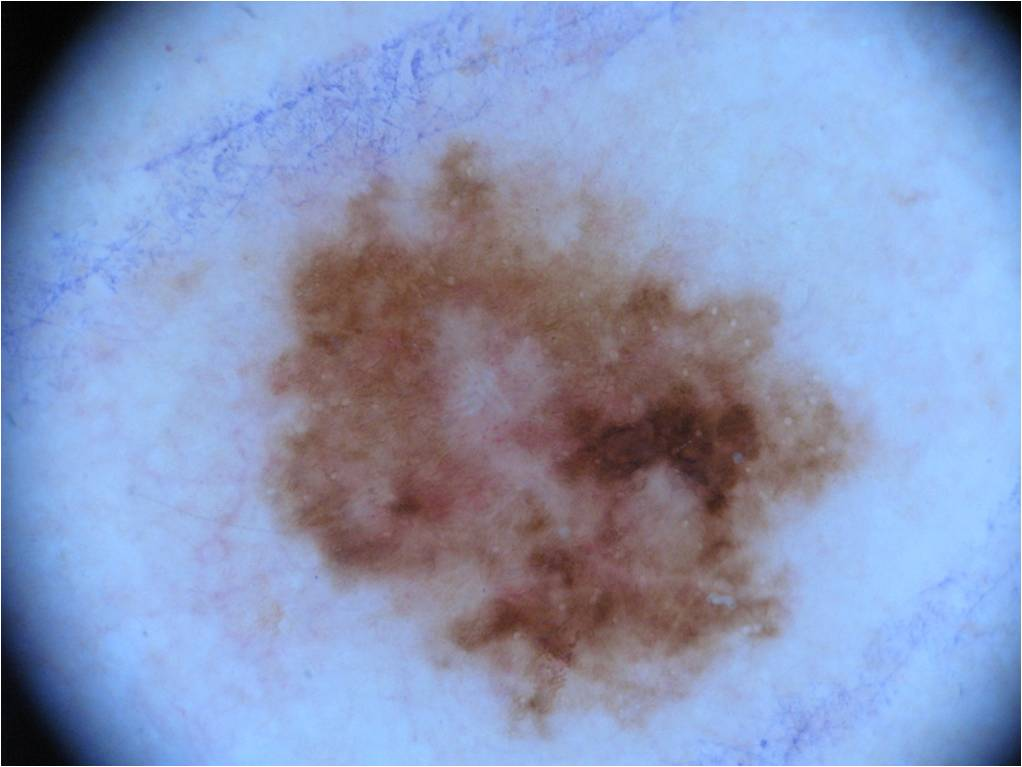
\includegraphics[width=.9\linewidth]{pictures/ISIC_0000002.jpg}  
		\caption{ISIC\_0000002: class 0}
		\label{fig:sub-second}
	\end{subfigure}
	
	\begin{subfigure}{.24\textwidth}
		\centering
		% include third image
		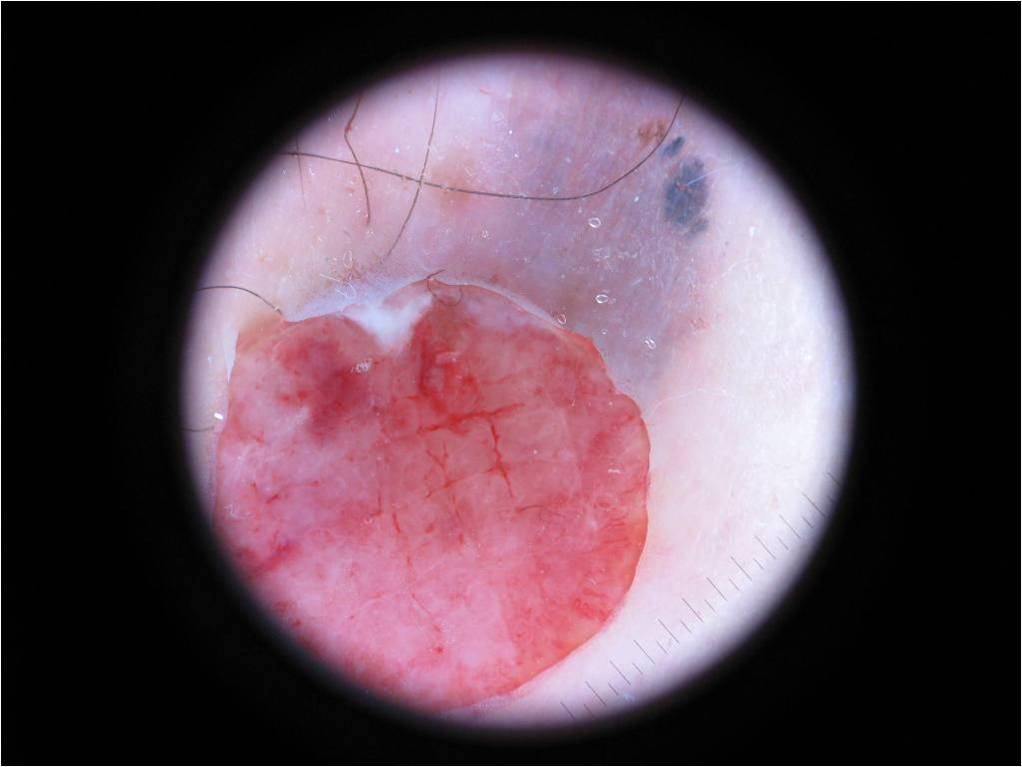
\includegraphics[width=.9\linewidth]{pictures/ISIC_0000004.jpg}  
		\caption{ISIC\_0000004: class 0}
		\label{fig:sub-third}
	\end{subfigure}
	\begin{subfigure}{.24\textwidth}
		\centering
		% include fourth image
		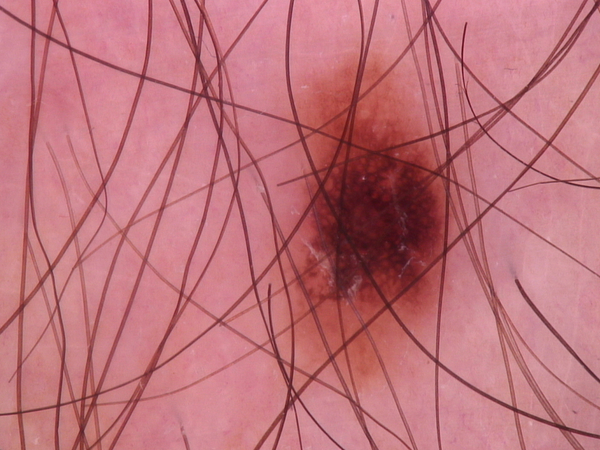
\includegraphics[width=.9\linewidth]{pictures/ISIC_0026767.jpg}  
		\caption{ISIC\_0026767: class 1}
		\label{fig:sub-fourth}
	\end{subfigure}
	\caption{Four images of the ``ISIC 2019: Training'' dataset.}
	\label{fig:dataset}
\end{figure}
%Only the skin lesion itself is interesting for the classification, not the normal skin around it or hair that covers the lesion.\\
There is also additional data for most images called meta data. This contains information of the age and gender of the belonging patient and the position of the skin lesion on the patients body. 
For the skin lesion classification we will present two different approaches: \\
In section \ref{sec:svm} we are using Support Vector Machine (SVM) for the classification. Therefor data preprocessing and feature extraction is necessary. These features describe the shape and texture of the image and are used as input data.
% This procedure can be seen in figure \ref{fig:intro_svm}.\\
In the following section \ref{sec:cnn} we are using a Convolutional Neural Network (CNN) for the classification. CNNs have become increasingly important in the domain of medical image analysis. Here the image itself is used as the input data. 
% This procedure can be seen in figure \ref{fig:intro_cnn}.
% \begin{figure}[ht!]
% 	%\centering
% 	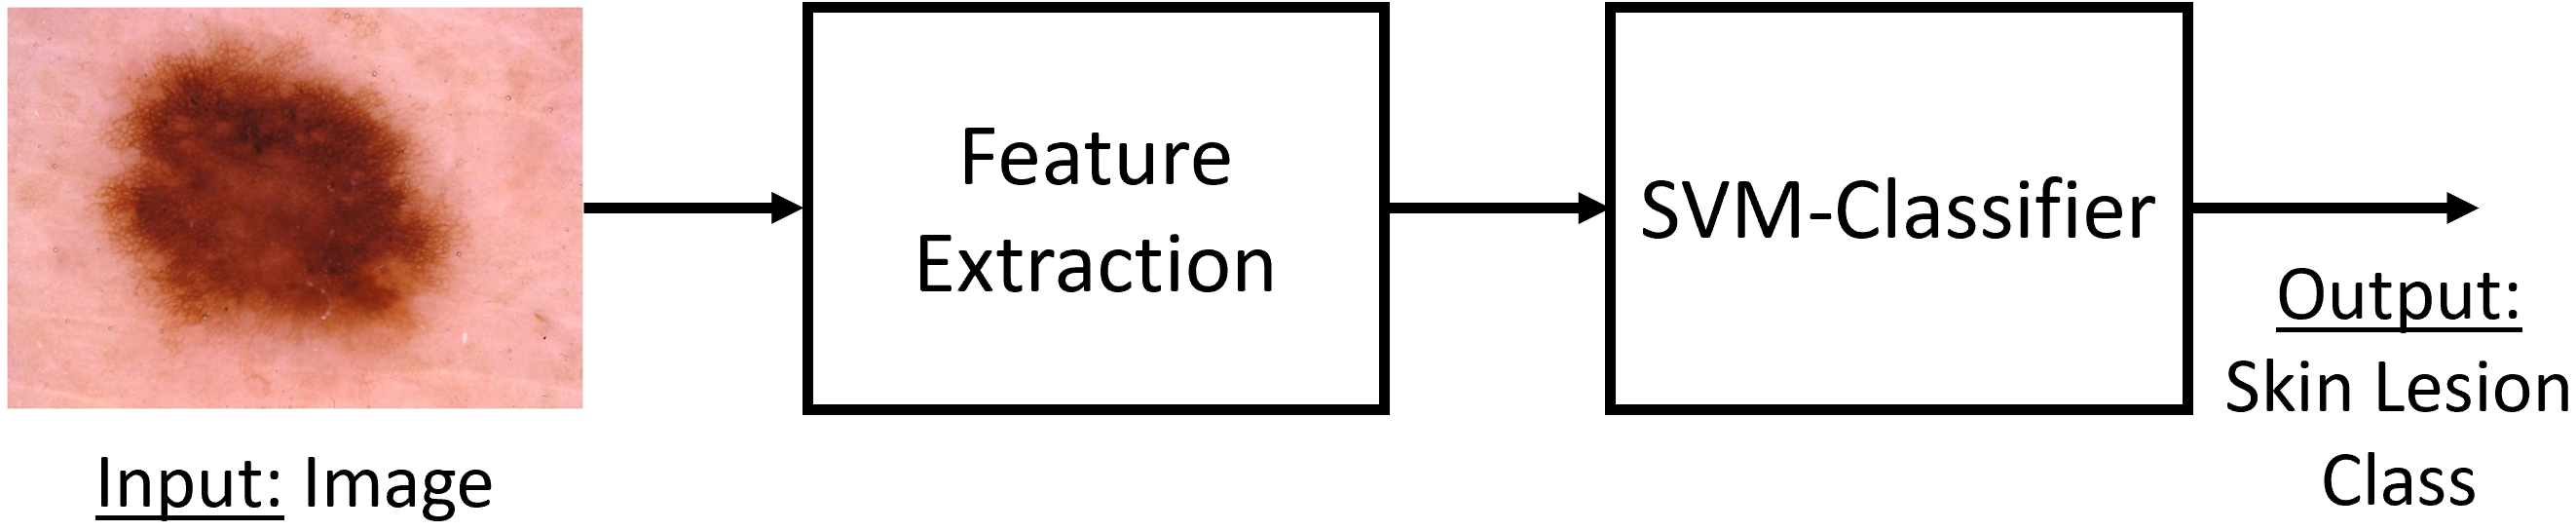
\includegraphics[height=1.8cm]{pictures/intro_01.png} 
% 	\caption{Classification with Support Vector Machine}
% 	\label{fig:intro_svm}
% \end{figure}
% \begin{figure}[ht!]
% 	%\centering
% 	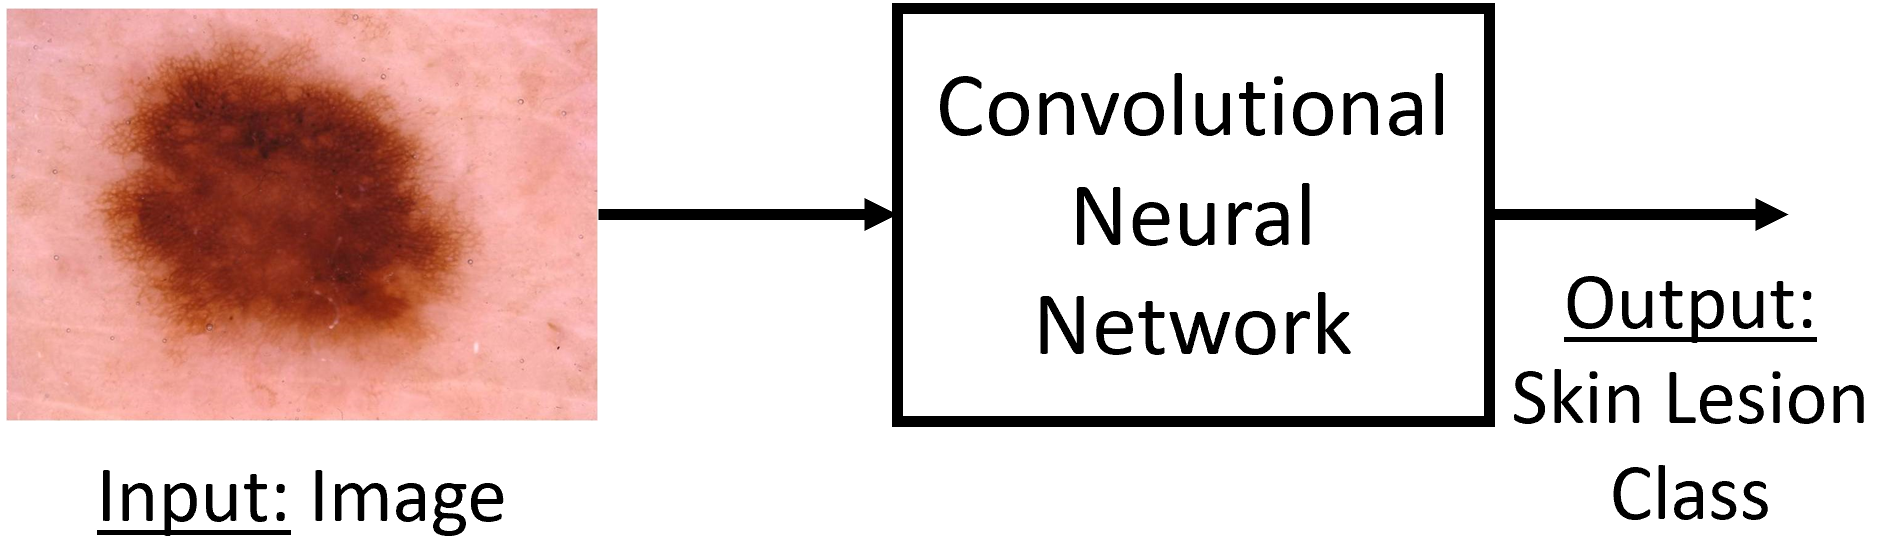
\includegraphics[height=1.8cm]{pictures/intro_02.png} 
% 	\caption{Classification with Convolutional Neural Networks}
% 	\label{fig:intro_cnn}
% \end{figure}
Furthermore we will investigate the prediction results by taking the additional meta data into account. 
One of the main challenges is the classification of the unknown class in the test dataset. Our approach for that is shown in section \ref{sec:unknown_data}.
In the last section \ref{sec:conclusion} we will discuss the two different approaches and summarize our results.

% !TEX root = Skin_Lesion_Classification_Using_Machine_Learning.tex

\section{Skin Lesion Classification Using Support Vector Machine [TN]}\label{sec:svm}
In this section we present a skin lesion classification approach by using Support Vector Machine (SVM). Therefor we first extract features out of the images that are then used as input data. Afterwards based on the extracted features we train and evaluate a SVM by making use of the Sklearn library \cite{scikit-learn}.   
\subsection{Feature Extraction [SPS]}

Feature extraction is the process of extracting relevant features that give information about the color,shape,texture etc. of the skin lesion.For extracting the features from the skin lesion it is mandatory to segment the skin lesion from the image and  then extract the features of the segmented lesion.In order to segment the lesion from the image , three segmentation techniques has been implemented.Initially an elliptical mask is applied to the image, and the skin lesion is extracted using the elliptical mask.Then features are extracted for the masked image and prepared as a data set.In the second segmentation technique which works on algorithm termed as watershed algorithm, the skin lesion is segmented based on peaks and valleys that are created based on the intensity gradient across the image.This kind of segmentation technique works really well on the images with no hair.But the images with hair , this type of segmentation did not work properly with hair as shown in the figure below.So after this segmentation technique the features are extracted and second data set is created.The final type of segmentation is done using k means clustering.It forms segmented regions using k clusters.The features for this kind of segmentation are extracted and then third data set is created.Based on the classification results from SVM, K means clustering technique found to give a better evaluation parameters like the high accuracy and high sensitivity.The features that were extracted after segmentation are listed as Moments, Huemoments,PCA features,Mean and Standard deviation of the color channels in the images,haralick features.
\subsubsection{Moments and Hu moments}
Image moments are a weighted average of image pixel intensities. Image moments capture information about the shape of a lesion in a binary image because they contain information about the intensity I(x,y) as well as position x and y of the pixels.The central moments are translation invariant. In other words, no matter where the lesion is in the image, if the shape is the same, the moments will be the same.       Hu Moments ( or rather Hu moment invariants ) are a set of 7 numbers calculated using central moments that are invariant to image transformations. The first 6 moments have been proved to be invariant to translation, scale, and rotation, and reflection. While the 7th moment’s sign changes for image reflection.
\subsubsection{Haralick features}
The basis for these features is the gray-level co-occurrence matrix . This matrix is square with dimension , where Ng is the number of gray levels in the image. Element [i,j] of the matrix is generated by counting the number of times a pixel with value i is adjacent to a pixel with value j and then dividing the entire matrix by the total number of such comparisons made. Each entry is therefore considered to be the probability that a pixel with value i will be found adjacent to a pixel of value j.

\subsubsection{PCA features}
PCA is essentially a method that reduces the dimension of the feature space in such a way that new variables are orthogonal to each other (i.e. they are independent or not correlated).By reducing the dimension of the feature space, we have fewer relationships between variables to consider  less likely to overfit the final model.
\begin{figure}
	\centering
	\includegraphics[width=1\linewidth]{pictures/Segmentation.png}  % You didn't upload the image, change if  required
	\caption{Different Types of Segmentation}
	\label{SVM_ROC}
\end{figure}

\subsection{Learning and Testing [TN]}
Based on the generated table with all extracted features and the corresponding skin lesion classes from the section above we use Sklearn to train the SVM. The classifier is set as follows: \textit{estimator =SVC(C=10, kernel='rbf', gamma='auto', probability=True, class\_weight=\glqq balanced\grqq, break\_ties=True, decision\_function\_shape='ovr')}. Here the regularization parameter C, the kernel, the degree of the polynomial kernel function and the gamma were tuned beforhand by trying out different combinations. To handle the unbalanced dataset we use class weights which are inversely proportional to its frequency in the datasat.\newline
The ROC curves which are created by plotting the true positive rate against the false positive rate at various threshold settings are shown in figure \ref{SVM_ROC}. In total we achieved a sensitivity score (true positive rate) of 51.558\%.
\begin{figure}
	\centering
	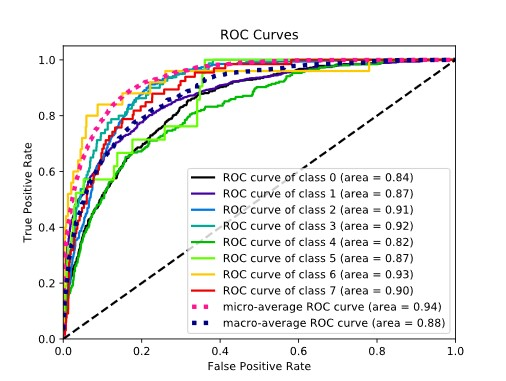
\includegraphics[width=1\linewidth]{pictures/SVM_ROC.jpg}  
	\caption{ROC Curves of the testing results}
	\label{SVM_ROC}
\end{figure}

\subsection{Consideration of Meta Data [TN]}
As already mentioned in the introduction there exsists additional data for most images called meta data. This contains information about the age, gender and the position of the skin lesion on the patients body. To make use of this additional data we convert each type into a one-hot vector and then attach all three vectors as additional input data. This improves the sensitivity score to 56.558\%.


% !TEX root = Skin_Lesion_Classification_Using_Machine_Learning.tex

\section{Skin Lesion Classification Using Convolutional Neural Networks [SE]}\label{sec:cnn}
For the second part of this project, we used convolutional neural networks (CNNs) to classify the images containing skin lesions. 
We apply transfer learning to pretrained networks on the ImageNet dataset. All training and testing was done on a Nvidia Tesla P100 with 16GB of video memory via Google Colab. The model and its input pipeline was developed using Tensorflow and evaluated using the same Sklearn functions as in section \ref{sec:svm}. 
\subsection{Architecture [SE]}
We use the EfficientNet models for our prediction pipeline.
The base model B0 uses the standart ImageNet input size of $224 \times 224$, the models B1 to B7 scale that base architecture and allow much larger input sizes. The models are scaled uniformly in resolution, width and depth. This helps them to achieve state of the art performance on standart datasets while being smaller and faster then conventional architectures \cite{tan2019efficientnet}.

In our work, we manly use the models B3 and B4 which have an input size of $300 \times 300$ and $380 \times 380$ respectively. 
Those models outperformed resnet and densenet architectures in initial testing by a large margin. While the step from model B2 to B3 brought a significant performance improvement, the results of B3 and B4 were relatively similar. Larger models could not be trained enough epochs because of resource constraints.

For our final model, we only add global average pooling and one dense classification layer with softmax activation to the pretrained network. We tried adding additional fully connected layers in between so that the number of neurons don't decrease so fast (1536 to 8 for B3) but this did not bring an improvement. 

\subsection{Data Augmentation and Input Strategies [SE]}\label{sub:cnn_input}
We used the tensorflow.data API to handle the large dataset efficiently. The batches of training data are automatically loaded in the background only when they are needed. 
To increase the variety of the dataset, we applied online data augmentation. These included randomly flipping and rotating images, as well as random changes in contrast brightness and hue. The larger images are then resized so that they fit the original size of the images from the HAM10000 dataset. The aspect ratio is kept at this operation. 
The input for the network consists of random crops of same size of these augmented images. 

A different strategy without augmentation is applied to the validation and test data. We use equally spaced crops as seen in the last years challenge \cite{gessert2018skin}.
Each image is divided into six by six overlapping cops. All crops share the size of of the training data. 

\subsection{Learning and Testing [SE]}
The training is done using the Adam optimizer. We apply a learning rate schedule to reduce the learning rate every 20 epochs. This helped the loss to decrease continuously during training procedure. 

The imbalanced dataset is handled as before by class weights. Every sample gets a weight assigned inversely proportional to its frequency in the dataset. The strategie proofed to be much more efficient in our tests than oversampling the less frequent classes. 
A batch size of 32 is used when ever possible and reduced for larger models to fit our GPU memory. 
In the first stage, we only train our final classification layer for 50 epochs. After that, the lower convolutional layer of the base model are unfrozen and also fitted to our dataset. This fine tuning of the more specialized convolution kernels gave us a big performance improvement. We train these layers using a low learning rate in several stages for an additional 75 epochs.  % #TODO more precise? 
Our final model was an ensemble of the B3 and B4 model. The predictions of both networks were averaged a the end. That technic improved the accuracy by tree percent points. The final model was able to archive a validation accuracy of 85.31\%. 

\subsection{Consideration of Meta Data [HBT]}

The Neural Networks with multiple inputs when the network require data from multiple sources or in different formats. For example, networks that require image data captured from multiple sensors at different resolutions. In many researches, the use of different type of data along with the image data for classification in deep learning has shown the considerable improvement in image classification\cite{love},\cite{melan}. The metadata is merged within the same pixel matrix of the image in each RGB layer which enriches the extraction of features, has shown significant improvement in accuracy in this research\cite{melan}. The image metadata is used nonparametrically to generate neighbourhoods of related images using Jaccard similarities, then used a deep neural network to blend visual information from the image and its neighbours in this research \cite{love}. McAuley and Leskovec pioneered the study of multilabel image annotation using metadata, and demonstrated impressive results using only metadata. In hope of improvement of accuracy mixed data approach is used.

% #TODO I'm sorry but that (above) aren't complete english sentences. I only partly get what you want to say

Including the metadata into the neural netwok is challenging. In contrast to the SVM based approach, the metadata is here in a different format then the image data. For that reason we created two separate networks and merged them. One branch is a Multi-Layer Perceptron (MLP) model that is designed to handle metadata and a second branch is a cnn for image data. Finally, these two branches are concatenated to have a final model for training.

The sex and position information of the metadat is converted to one-hot numpy arrays, the age is used as an numerical value. The MLP model consists of 4 layers with relu activation function with (128,64,32,8) neurons respectively. It has two inputs, age and sex. 
The conventional customized CNN model with 3 layers, with 3x3 filter size and (16,32,64) depth respectively and stride of 2 is chosen. Padding is done to the images to maintain the same length. Another CNN model with EfficientNet B4 for transfer learning followed by GlobalMaxPooling and 2 Dense layers with (512,8) neurons with SoftMax activation to the pretrained network. The transfer learning is performed using both the EfficientNet model and conventional CNN for better approximation of expected outputs. The cnn is trained the same way as before. 

\begin{figure}[h]
    \centering
    % include first image
    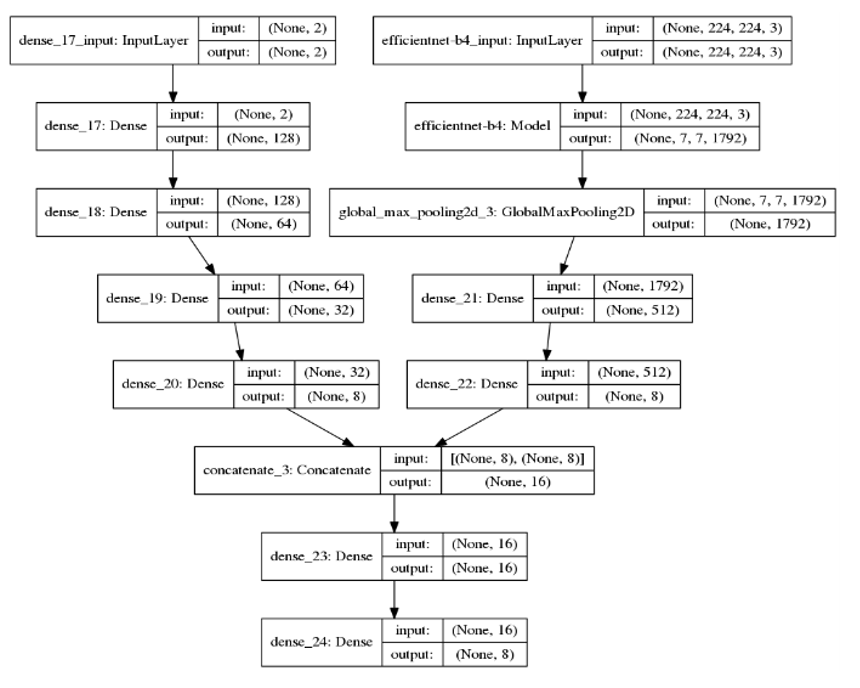
\includegraphics[width=.75\linewidth]{pictures/model.PNG}  
    \caption{Multi \- Input model that includes both CNN and MLP branches to handle mixed data.}
    \label{fig:model}
\end{figure}
% #TODO this picture is way to small to read

Figure \ref{fig:model} shows the Multi-Input model which combines both networks. 

Due to technical problems concerning the connection of tensorflow and keras, we could not use the image input pipeline described in section \ref{sub:cnn_input}. 
A validation accuracy of 53.63\% was achieved using the Multi-Input model. There is huge requirement of improvement in image data pre-processing techniques, hyper-parameter tuning, extracting features from image related to metadata for multi-input model as compared CNN model by considering only image data. Since the images are loaded using Open CV at onetime without using any Data Loading Pipeline, the training was taking very long time for each epoch. Normalizing is done at once for a whole image array is not efficient way and proved by experimenting it.
The accuracy is better for CNN model with a pre-trained EfficientNet model. Since the computational problems caused by OpenCV library in high resolution image data loading as input to multi-input model requires implementation of precise image processing techniques and a precise regularization with the loss obtained from model. The learning has to be regulated by considering metadata with respect to image data. Image augmentation and few other techniques may enhance the accuracy.  

% #NOTE I included most of it in the cnn section, change it back if you don't like it
% % !TEX root = Skin_Lesion_Classification_Using_Machine_Learning.tex

% #TODO this is very long, check for redundant parts

\section{Skin Classification using Convolutional Neural Network and Metadata [HBT]}\label{sec:metadata_cnn}
The Neural Networks with multiple inputs when the network require data from multiple sources or in different formats. For example, networks that require image data captured from multiple sensors at different resolutions. In many researches, the use of different type of data along with the image data for classification in deep learning has shown the considerable improvement in image classification\cite{love},\cite{melan}. The metadata is merged within the same pixel matrix of the image in each RGB layer which enriches the extraction of features, has shown significant improvement in accuracy in this research\cite{melan}. The image metadata is used nonparametrically to generate neighbourhoods of related images using Jaccard similarities, then used a deep neural network to blend visual information from the image and its neighbours in this research \cite{love}. McAuley and Leskovec pioneered the study of multilabel image annotation using metadata, and demonstrated impressive results using only metadata. In hope of improvement of accuracy mixed data approach is used.
\subsection{Data Pre-processing and Data loading [HBT]}
The meta data which is numerical data consists of age, gender and the position of the skin lesion on the patient’s body. The sex data is one-hot encoded like female as 1, male as 0 and empty spaces as 3, to improve the data pre-processing step. The age data is already numerical value, so it is taken without one hot encoding. The loading of csv files into data frame and processed. The image data splitting is performed by customised function, where the whole image data is splitting into training data and testing data. The meta data is also splitting using the same function with respect to image data and mapping of metadata to corresponding image data is performed by using image file name. The listed pre-processing tasks are performed using Pandas library.

Even though the Keras API is capable of handling higher resolution images as input, the use of OpenCV library provides few computational problems to handle the high-resolution images. The larger image dataset is handled by resizing the images. So smaller resolution images are given as input to the CNN model. The use of OpenCV library functions to load images and original images are very large, so resized the image to desired size i.e,224 x 224 x 3. The image data is converted to NumPy array format for easy computation. Normalization is done to scale the values to have a similar data distribution and nullify the effect of large values. Since the model is handling two different types of data, which requires separate pre-processing steps including scaling, normalization, and feature engineering. This is extremely challenge encountered in recent researches.
\subsection{Multi-Input Model Architecture [HBT]}
\begin{figure}[h]
    \centering
    % include first image
    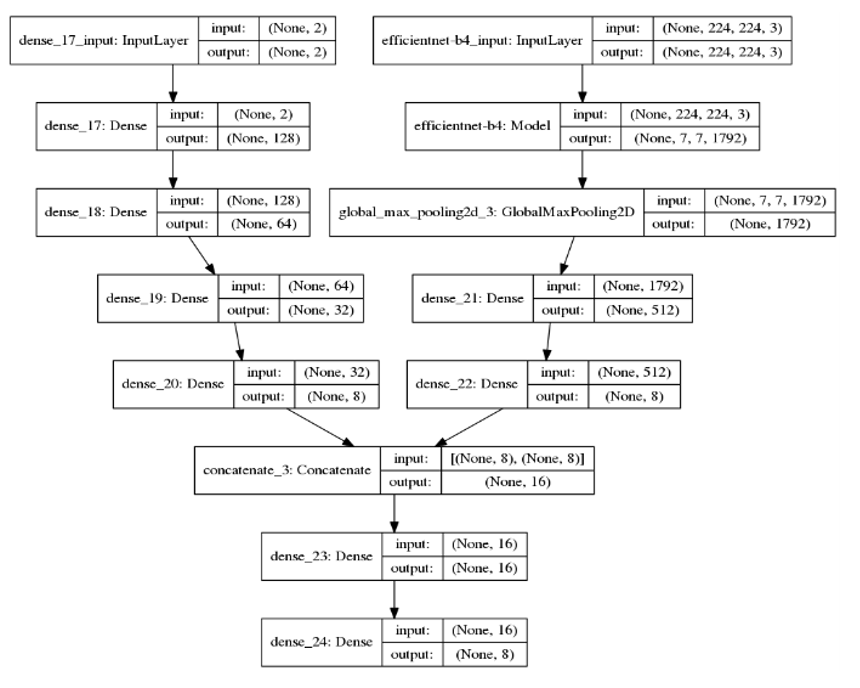
\includegraphics[width=.75\linewidth]{pictures/model.PNG}  
    \caption{Multi - Input model that includes both CNN and MLP branches to handle mixed data.}
    \label{fig:model}
\end{figure}
% #TODO this picture is way to small to read
The multi-input model is built to handle both image input and metadata which is a numerical data input is challenging task. The Keras API is used to build the multi input model, there is a requirement of two branches. First branch is a Multi-Layer Perceptron (MLP) model is designed to handle metadata and second branch is Convolution Neural Networks (CNN) for image data. Finally, these two branches are concatenated to have final model for training. The process of scaling is random in conventional CNN and is proved not be efficient. The reuse of scaling technique along single dimension alone can improve the accuracy, but model will quickly saturate\cite{tan2019efficientnet}. The transfer learning is performed to save computational time by a pre-trained CNN model EfficientNet, which involves systematic and principled scaling of depth, width and Resolution performs better than all the existing deep learning networks used in CNN \cite{tan2019efficientnet}.
MLP model consists of 4 layers with relu activation function with (128,64,32,8) neurons respectively. With 2 inputs age and sex respectively.The conventional customised CNN model with 3 layers, with 3x3 filter size and (16,32,64) depth respectively and stride of 2 is chosen. Padding is done to the images to maintain the same length. Another CNN model with EfficientNet B4 for transfer learning followed by GlobalMaxPooling and 2 Dense layers with (512,8) neurons with SoftMax activation to the pretrained network. The transfer learning is performed using both the EfficientNet model and conventional CNN for better approximation of expected outputs. 
\subsection{Training[HBT]}
The model is trained on a Nvidia Tesla P100 with 16GB of video memory via Google Colab. The model is developed using Keras API. We combined the MLP and CNN model using Concatenate function from Keras API to combine these two sub models. Now for final we provide the processed meta data as well as normalized image data array. The model compilation uses ‘Adam’ as optimizer and ‘accuracy’ as metric. The multi-class classification requires ‘categorical\_crossentropy’ as loss function. 
Training is done with image of 224 of height,224 of width, for 30 epochs and batch size of 32. In case of CNN with transfer learning, last 125 layers are unfreezed and fine-tuned them to be trainable to fit for our classification model and observe specific features related the image data given. First few layers of CNN are freezed to make them learn abstract features like edges, contours and many more features.

\subsection{Learning and conclusion}

Training accuracy of 54.52\% and Validation accuracy of 53.63\% was achieved using Multi-Input model. There is huge requirement of improvement in image data pre-processing techniques, hyper-parameter tuning, extracting features from image related to metadata for multi-input model as compared CNN model by considering only image data. Since the images are loaded using Open CV at onetime without using any Data Loading Pipeline, the training was taking very long time for each epoch. Normalizing is done at once for a whole image array is not efficient way and proved by experimenting it. 
 The accuracy is better for CNN model with a pre-trained EfficientNet model. Since the computational problems caused by OpenCV library in high resolution image data loading as input to multi-input model requires implementation of precise image processing techniques and a precise regularization with the loss obtained from model. The learning has to be regulated by considering metadata with respect to image data. Image augmentation and few other techniques may enhance the accuracy.  



% !TEX root = Skin_Lesion_Classification_Using_Machine_Learning.tex

\section{Handling of Unknown Data [SE]}\label{sec:unknown_data}

As mentioned in section \ref{sec:introduction}, the test dataset contains images that don't belong to any of the categories of the training dataset. There is no information about the number of unknown images, the only given information is, that these images still show human skin and skin lesions. The performance of our models on the test dataset was not revealed before the submission deadline. That conditions made it hard to tune the testset classification accuracy. 

The automated evaluation system for this challenge required for each image a vector where each element is equal to the estimated probability for the respective class. In contrast to the real ISIC 2019 challenge, this vector is supposed to sum up to $1$. For that reason it was obvious to use a softmax activation function for the neural network approach. We assumed that the maximum value of the predicted class probabilities (referred to as confidence in the following) will be low for images of the unknown category. Literature sows that this assumption is not necessary true \cite{softmax_conf}. To test if this approach is still usable in this situation, we set all images showing basal cell carcinoma (class $2$) to unknown and trained the model on the remaining seven categories. 

\begin{figure}[h]
    \centering
    % include first image
    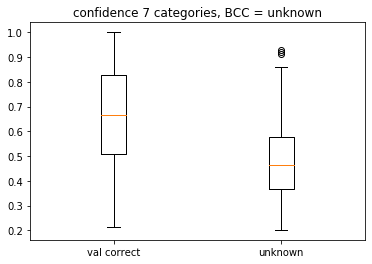
\includegraphics[width=.75\linewidth]{pictures/box_unknown.png}  
    \caption{comparison of distribution of confidence for known and unknown images}
    \label{fig:box_unknown}
\end{figure}
% #TODO maybe use hist or create better plot
Figure \ref{fig:box_unknown} shows the result of this test. The bar for "val correct" referrers to the confidence values for the correctly classified images in the validation dataset, "unknown" to the confidence for the images of the class that was set to unknown. It can be seen, that our assumption holds for this test. The confidence for unknown images is in average significantly lower. Both classes are however not perfectly separated. With no additional information it is not easy to assign a threshold for the confidence under which the lesion is assumed to be unknown. With no feedback for the performance on the test dataset we didn't see any evaluation method that would allow us to optimize this hyperparameter. 
Given the time constraints however, we decided that this approach is the best method available for us to handle the unknown class. 

We wanted to use this approach also in phase one using a SVM but the SVC class in sklearn does only predict classes and does not output probabilities for them. The \verb|predict_proba| method wich can for other classifiers output probability estimates was not applicable for SVMs. It uses Platt scaling and internal cross validation to create probabilities \cite{scikit-learn}. However they are not consistent with the normal class estimations and produced much worse results. For that reason we followed the advice in the documentation and used the values of the decision function for our confidence threshold. 

% !TEX root = Skin_Lesion_Classification_Using_Machine_Learning.tex

\section{Discussion and Conclusion [SE]}\label{sec:conclusion}

One of the most important factors for the final score of the 2019 ISIC challenge was the handling of unknown data. At the time of writing, we do not have a performance score for the complete test dataset. An email asking for scoring was not was not answered. Our best evaluation score of 85.31\% for the deep learning approach is in the top range of evaluation scores that were claimed by participants of the ISIC challenge in there papers. The performance on the test dataset was in general much lower. 
With that limitations, we can not rate if our models would achieve good final results and are able to precisely detect the unknown images. 

% #TODO needs to be reviewed, this is just a draft

We were able to achieve much better results using deep-learning and CNNs than with the simple classifiers. However it could not be determined if the limiting factor was the feature extraction or the support vector machine. A downside of the CNN based approach is the resource usage. We trained the SVM on a single core of a desktop CPU for under ten minutes while the CNN required several hours of training on an enterprise grade GPU. The required time for image prediction using the trained model scaled the same way. This aspect can become a problem when deploying the model for practical use as it enforces a powerful cloud computing infrastructure. 

We belief that an automated machine learning based system for skin lesion classification could be applied in a medical context. The main use for a product like this would be an assistance to human doctors. To little guarantees can be given in order to convert this models in stand allone diagnostics systems. In last years ISIC challenge which had no unknown category, the majority of algorithms was able to beat human experts \cite{TSCHANDL2019938}. This experiment has not yet been done for the current challenge. Together with legal challenges to certify a medical product, we conclude that a hybrid approach of algorithm and human would be the best usage. 	

Out of distribution detection is an active filed of research. Some theoretical problems of a softmax confidence based approach like adversarial attacks \cite{lee2018simple} are not relevant for this problem. However state of the are methods are usually more complex and can deliver more reliable results. These include diffrent loss functions and calibration or apply a two stage approach. In that case a unsupervised  model is used to detect unknown images before the main model classifies the remaining ones \cite{daxberger2019bayesian}. 

% #TODO (hypothetical) future work
% scaling high res images down is a waste of information, include some preprocessing in cnn (see challenge papers), better use of metadata
In our input pipeline for the deep-learning approach, we scale down larger images to match the size of the HAM1000 dataset. This is a waste of information. In future work one should try to scale up the lower resolution images insteat. Given sufficient hardware, it would be possible to use larger EfficientNet Models and take larger crops. 

Appart from the segmentation in the first phase, we did not apply and preprocessing other then the described data augmentation. It has been shown, that techniques like Color Constancy can improve the robustness and accuracy, specially when dealing with data from diffrent sources \cite{color}. 
The inclusion of metadata improved our results while using a support vector machine. Applying it to a convolutional neural network turned out to be hard. Technical problems hindered us from achieving good results here. Nevertheless we do see potential to improve the results in the inclusion and would continue trying to use them efficiently.  

% include sources in bibtex style (available at most databases) in the sources.bib file

\bibliographystyle{ieeetr}
\bibliography{sources}
\end{document}
